Dla każdej operacji zostanie wczytany ten sam obraz i zamieszczone poniżej zrzuty ekranu będą prezentowały podgląd zdjęcia przed i po, a także panel z parametrami.
Zaimplementowano najpopularniejsze \cite{mostpop} metody, które pasowały do obecnych założeń projektu - operacja powinna przetwarzać obraz i zwracać obraz jako wynik.
\subsubsection{Blur}
\begin{figure}[H]
    \centering
    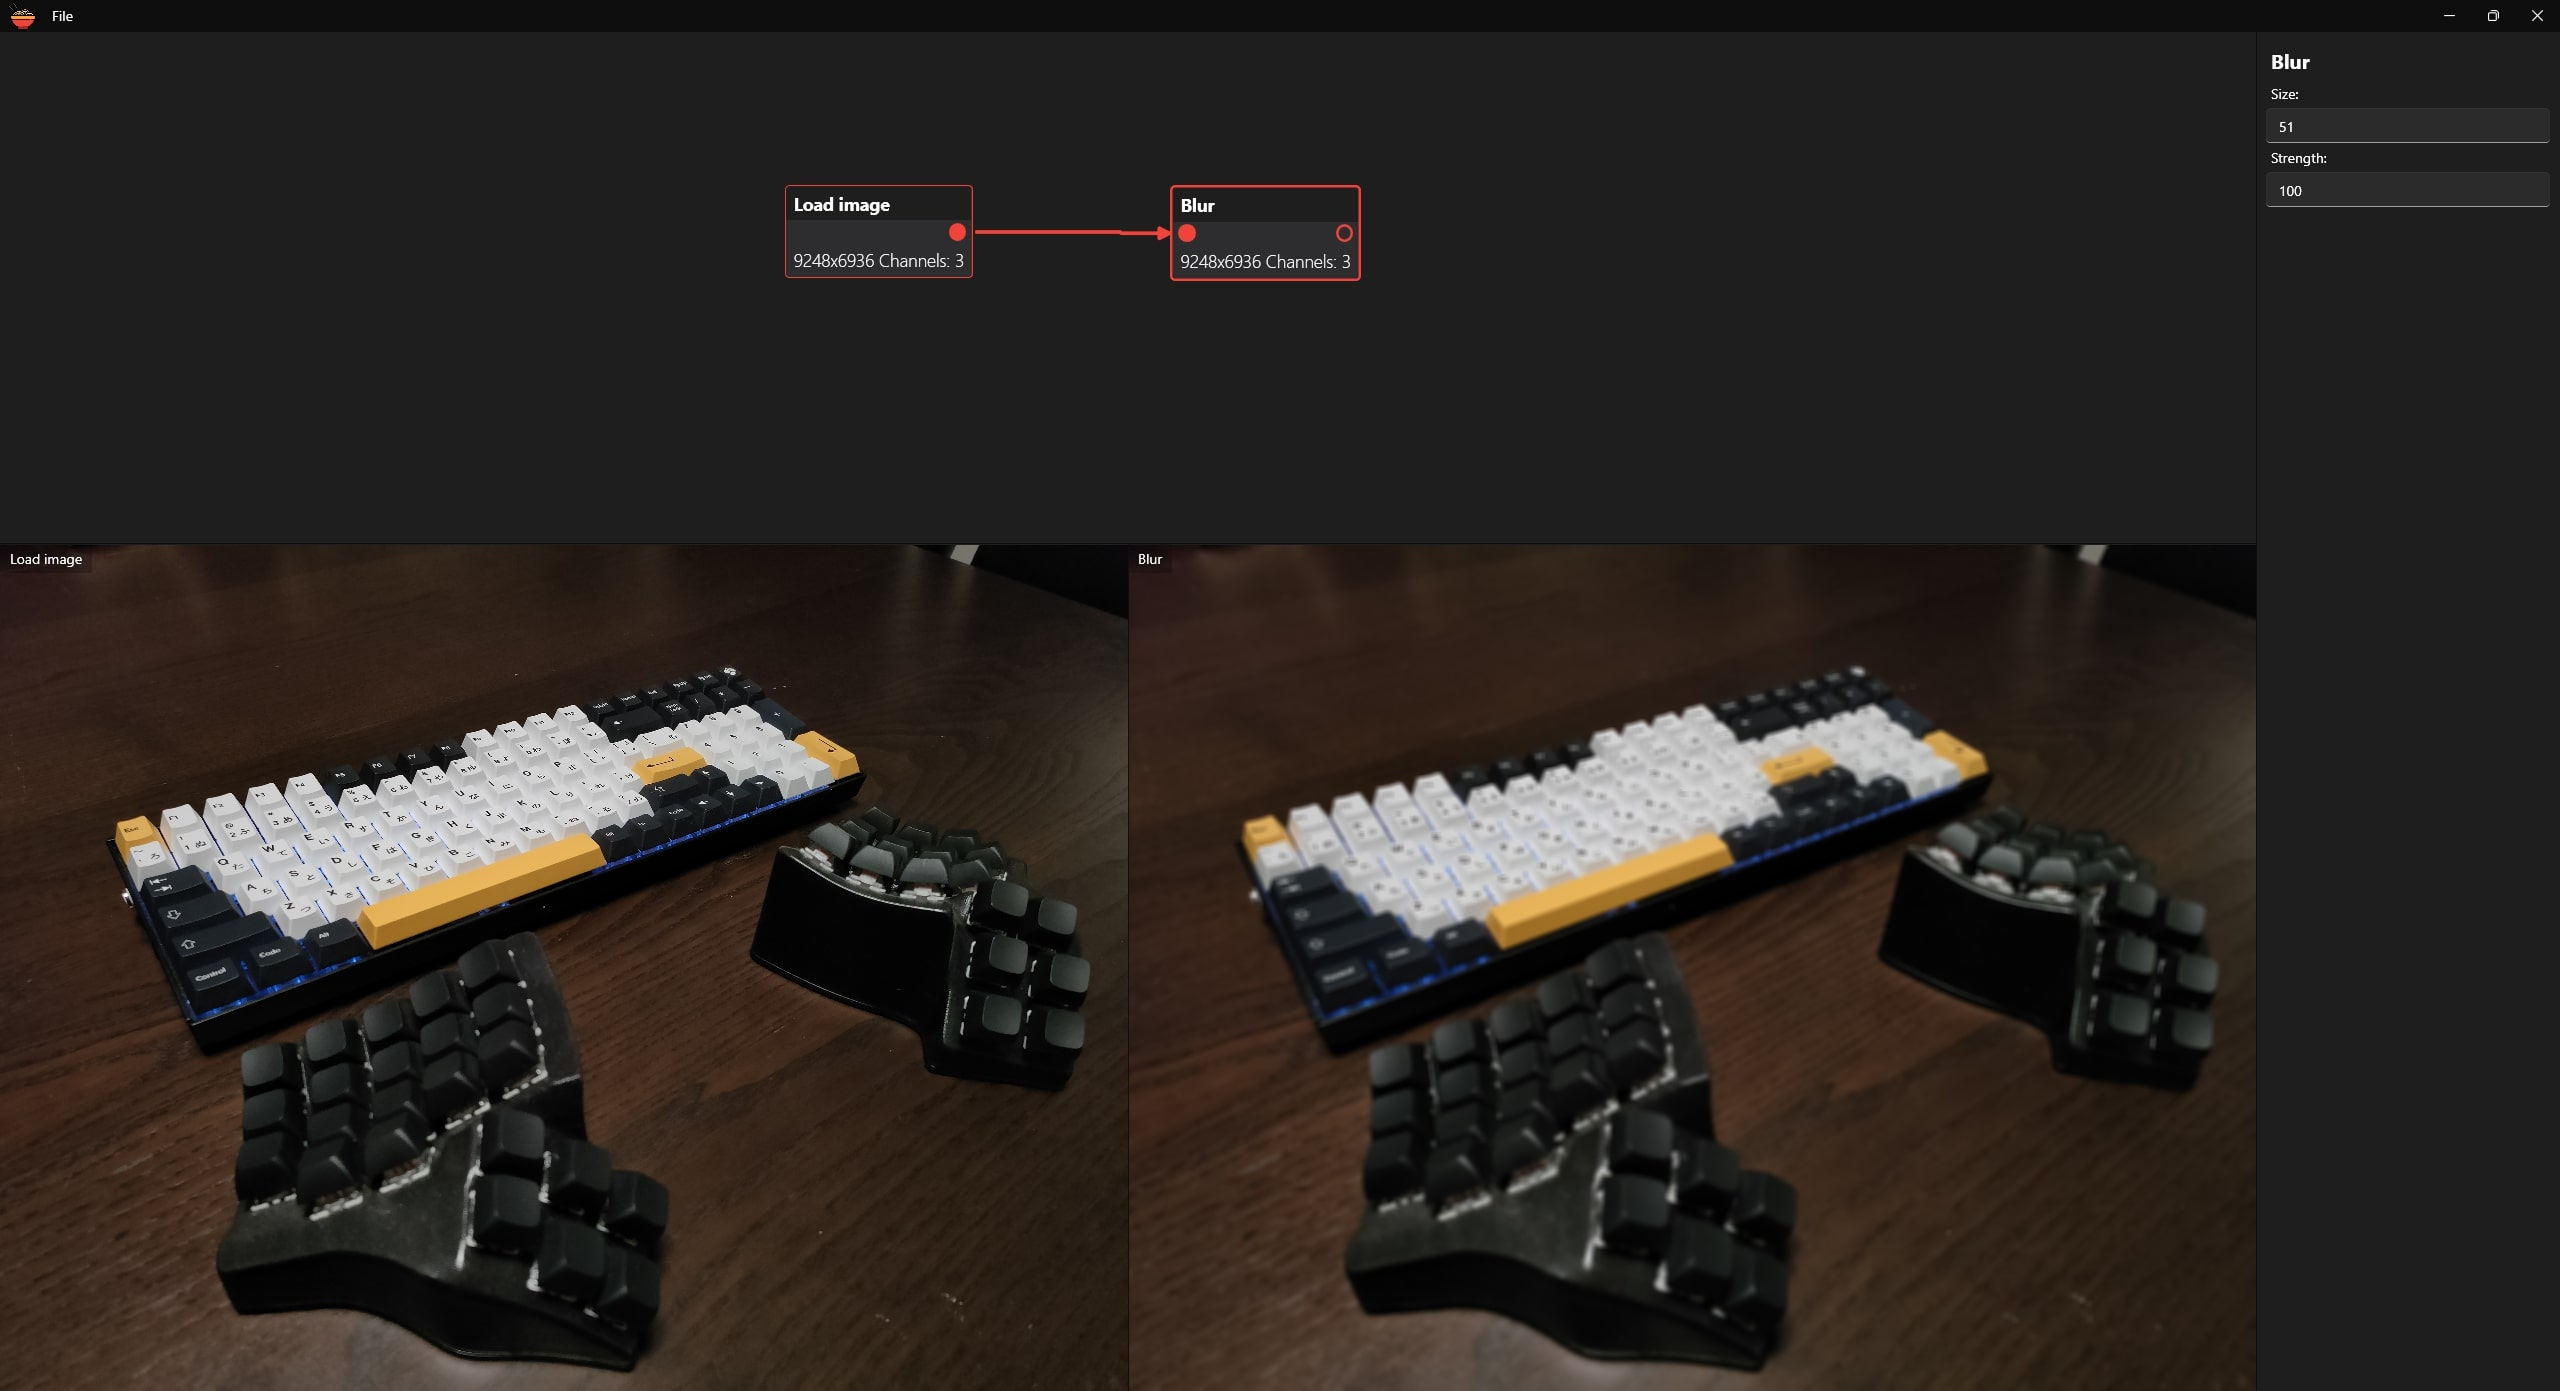
\includegraphics[width=1\linewidth]{images/Picture22.jpg}
    \caption{Operacja \textit{Blur}. Opracowanie własne.}
    \label{fig:blur}
\end{figure}

Zaimplementowana w oparciu o \textit{Gaussian Blur} \cite{gauss}. Parametr \textit{Size} musi być nieparzysty ponieważ opisuje on rozmiar maski na podstawie której wartość piksela jest uśredniana - potrzeby jest środek. \textit{Strength} opisuje natomiast odchylenie standardowe jakie będzie zastosowane przy przeprowadzaniu operacji.

\subsubsection{ChangeColorspace}

\begin{figure}[H]
    \centering
    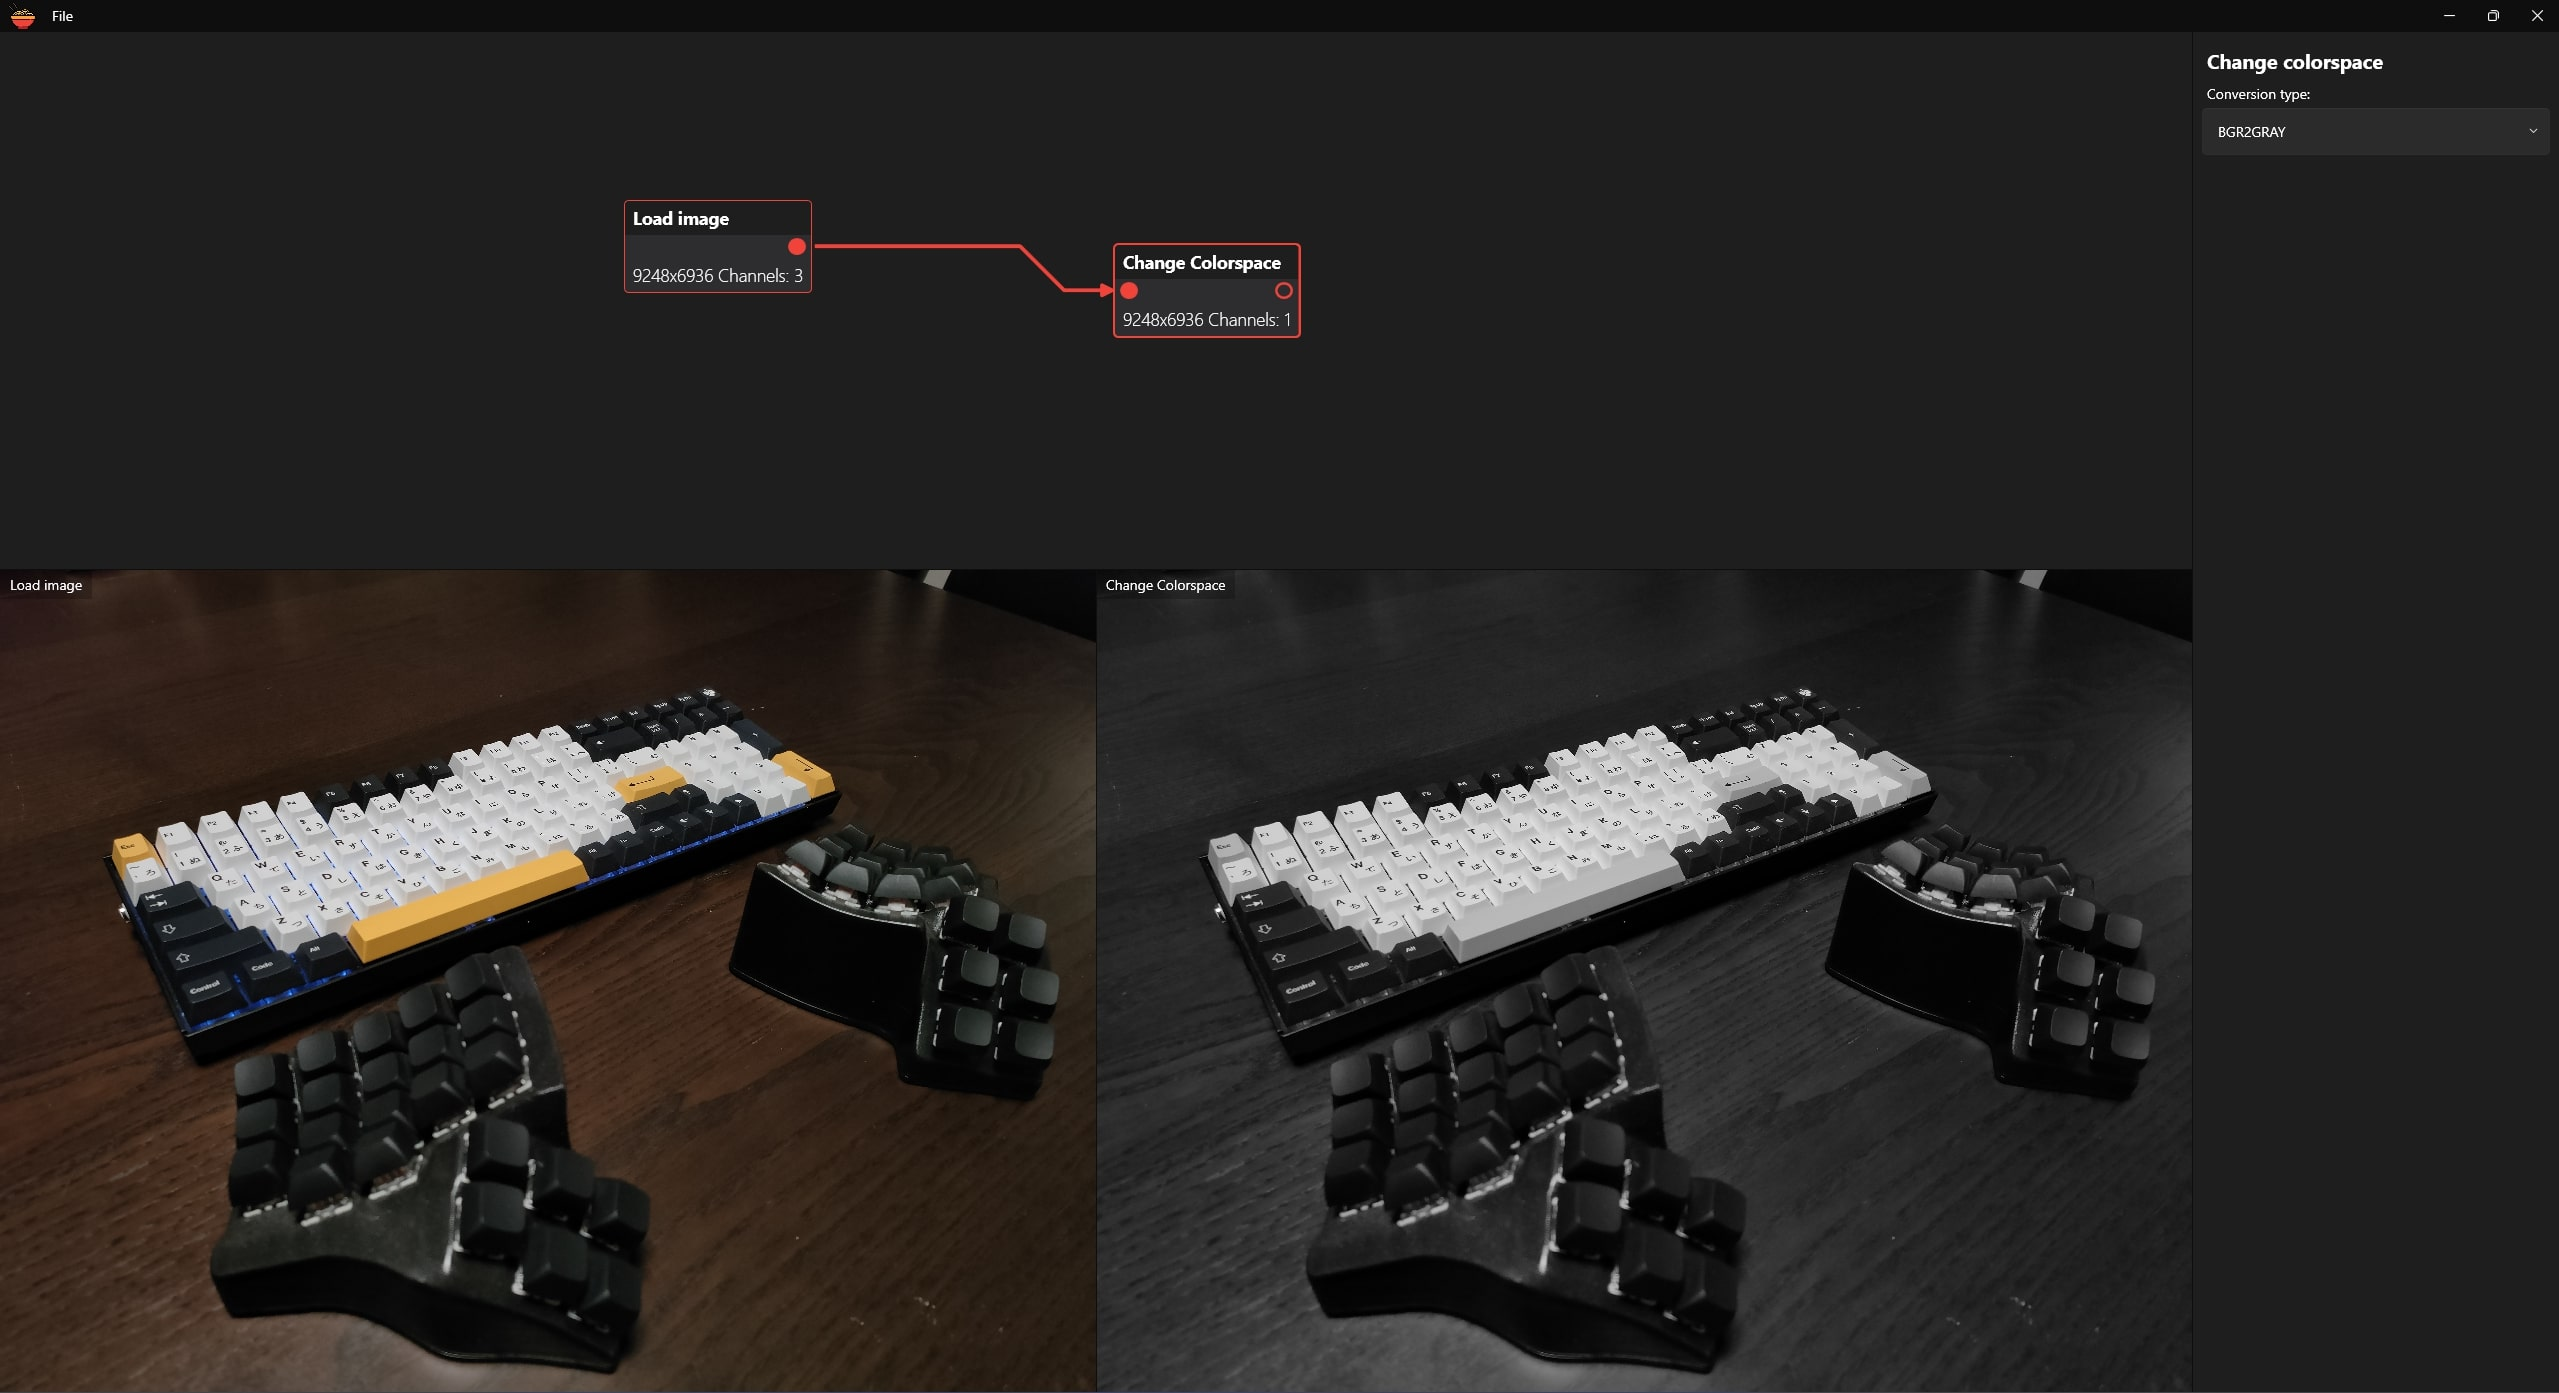
\includegraphics[width=1\linewidth]{images/Picture23.jpg}
    \caption{Operacja \textit{ChangeColorspace}. Opracowanie własne.}
    \label{fig:colorconv}
\end{figure}

Jest to funkcja \textit{CvtColor} \cite{cvtcol}. Konwertuje ona przestrzeń kolorów obrazu i dopasowuje ilość kanałów.
Jej jedynym parametrem jest kod z rodzajem konwersji np. \textit{BGR2GRAY} oznaczający przejście ze zwykłego kolorowego zdjęcia na biało-czarne.

\subsubsection{Crop}

\begin{figure}[H]
    \centering
    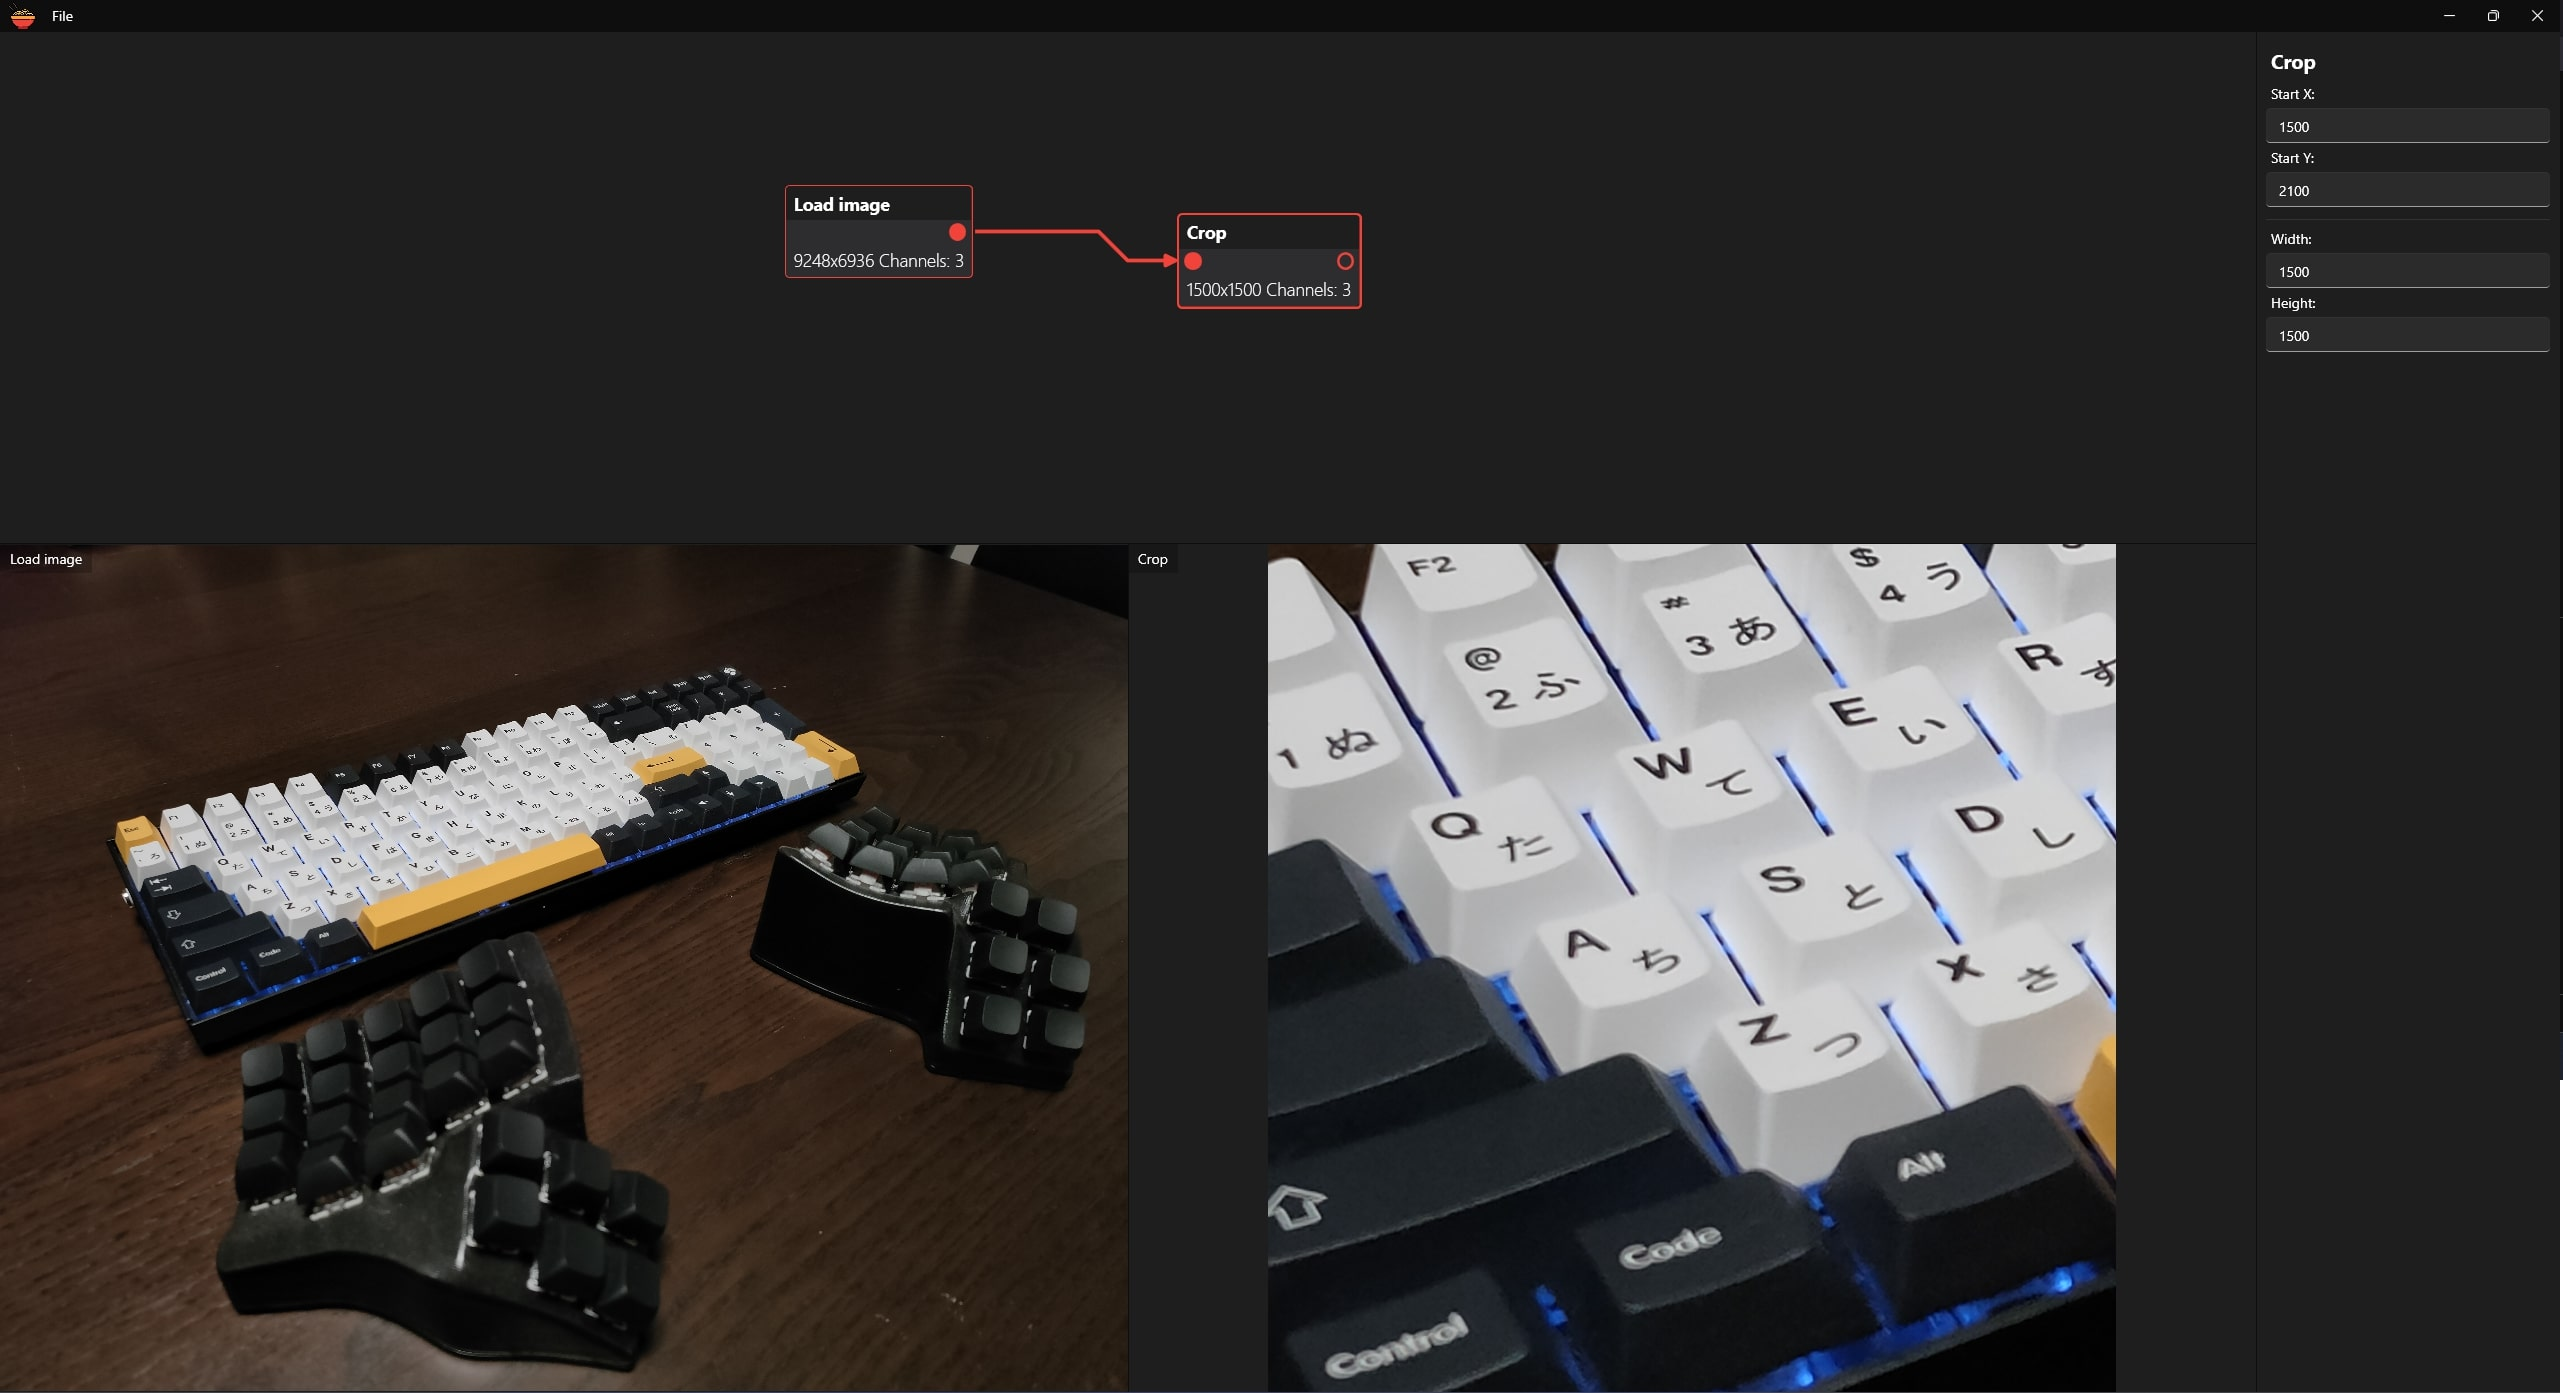
\includegraphics[width=1\linewidth]{images/Picture24.jpg}
    \caption{Operacja \textit{Crop}. Opracowanie własne.}
    \label{fig:crop}
\end{figure}

Operacja przycinania (ang. \textit{crop}) jest realizowana poprzez wykorzystanie koordynatów początkowych, a także określenia wysokości i szerokości nowo tworzonego prostokąta. Po zdefiniowaniu tych czterech parametrów, użytkownik uzyskuje nowy obraz, którego wymiary odpowiadają podanym wartościom, a punkt początkowy określa jego położenie w ramach oryginalnego obrazu.

\subsubsection{EdgeDetect}

\begin{figure}[H]
    \centering
    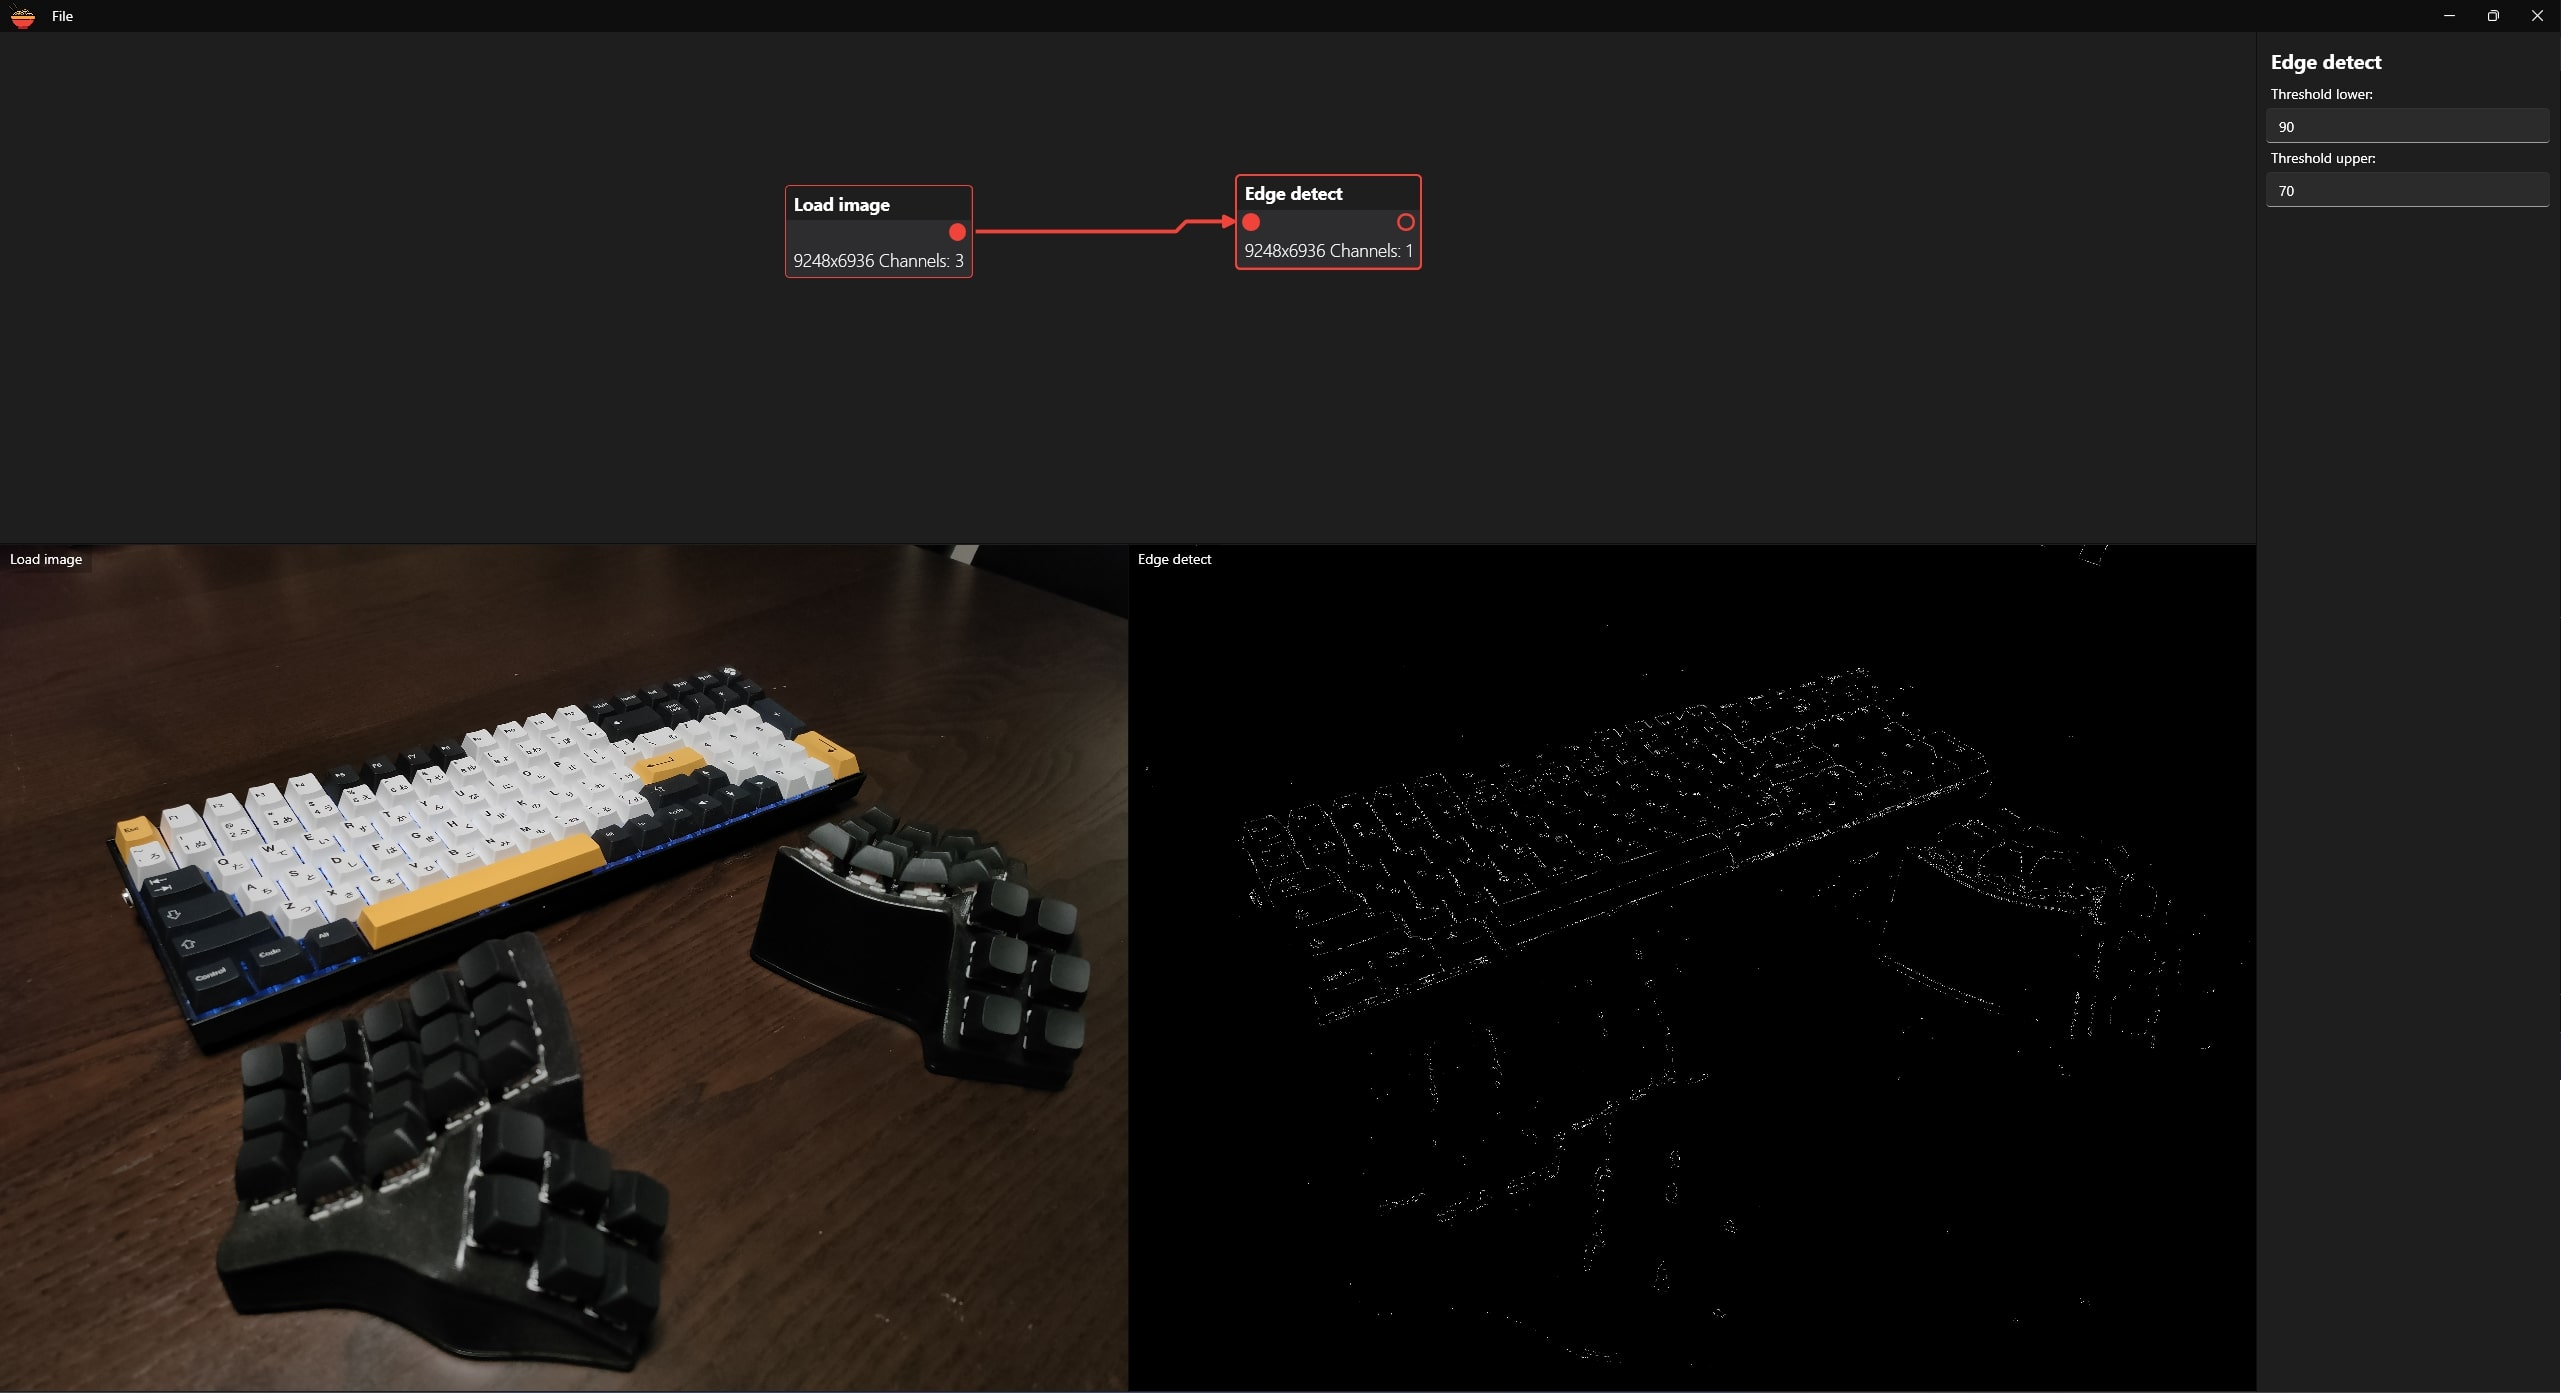
\includegraphics[width=1\linewidth]{images/Picture25.jpg}
    \caption{Operacja \textit{EdgeDetect}. Opracowanie własne.}
    \label{fig:edgeDetect}
\end{figure}  

Metoda \textit{Canny} \cite{canny} to jeden z kilku dostępnych algorytmów wykrywania krawędzi. Jako parametry wejściowe należy podać niższy i wyższy próg akceptacji.
Jeżeli krawędź jest mało wyraźna zostaje odrzucona przez algorytm. 
Wartości powyżej drugiego parametru są uznawane za krawędź, a te które są pomiędzy zostają włączone do wyniku jako element łączący krawędzie jeżeli taki jest. 

\subsubsection{Resize}

\begin{figure}[H]
    \centering
    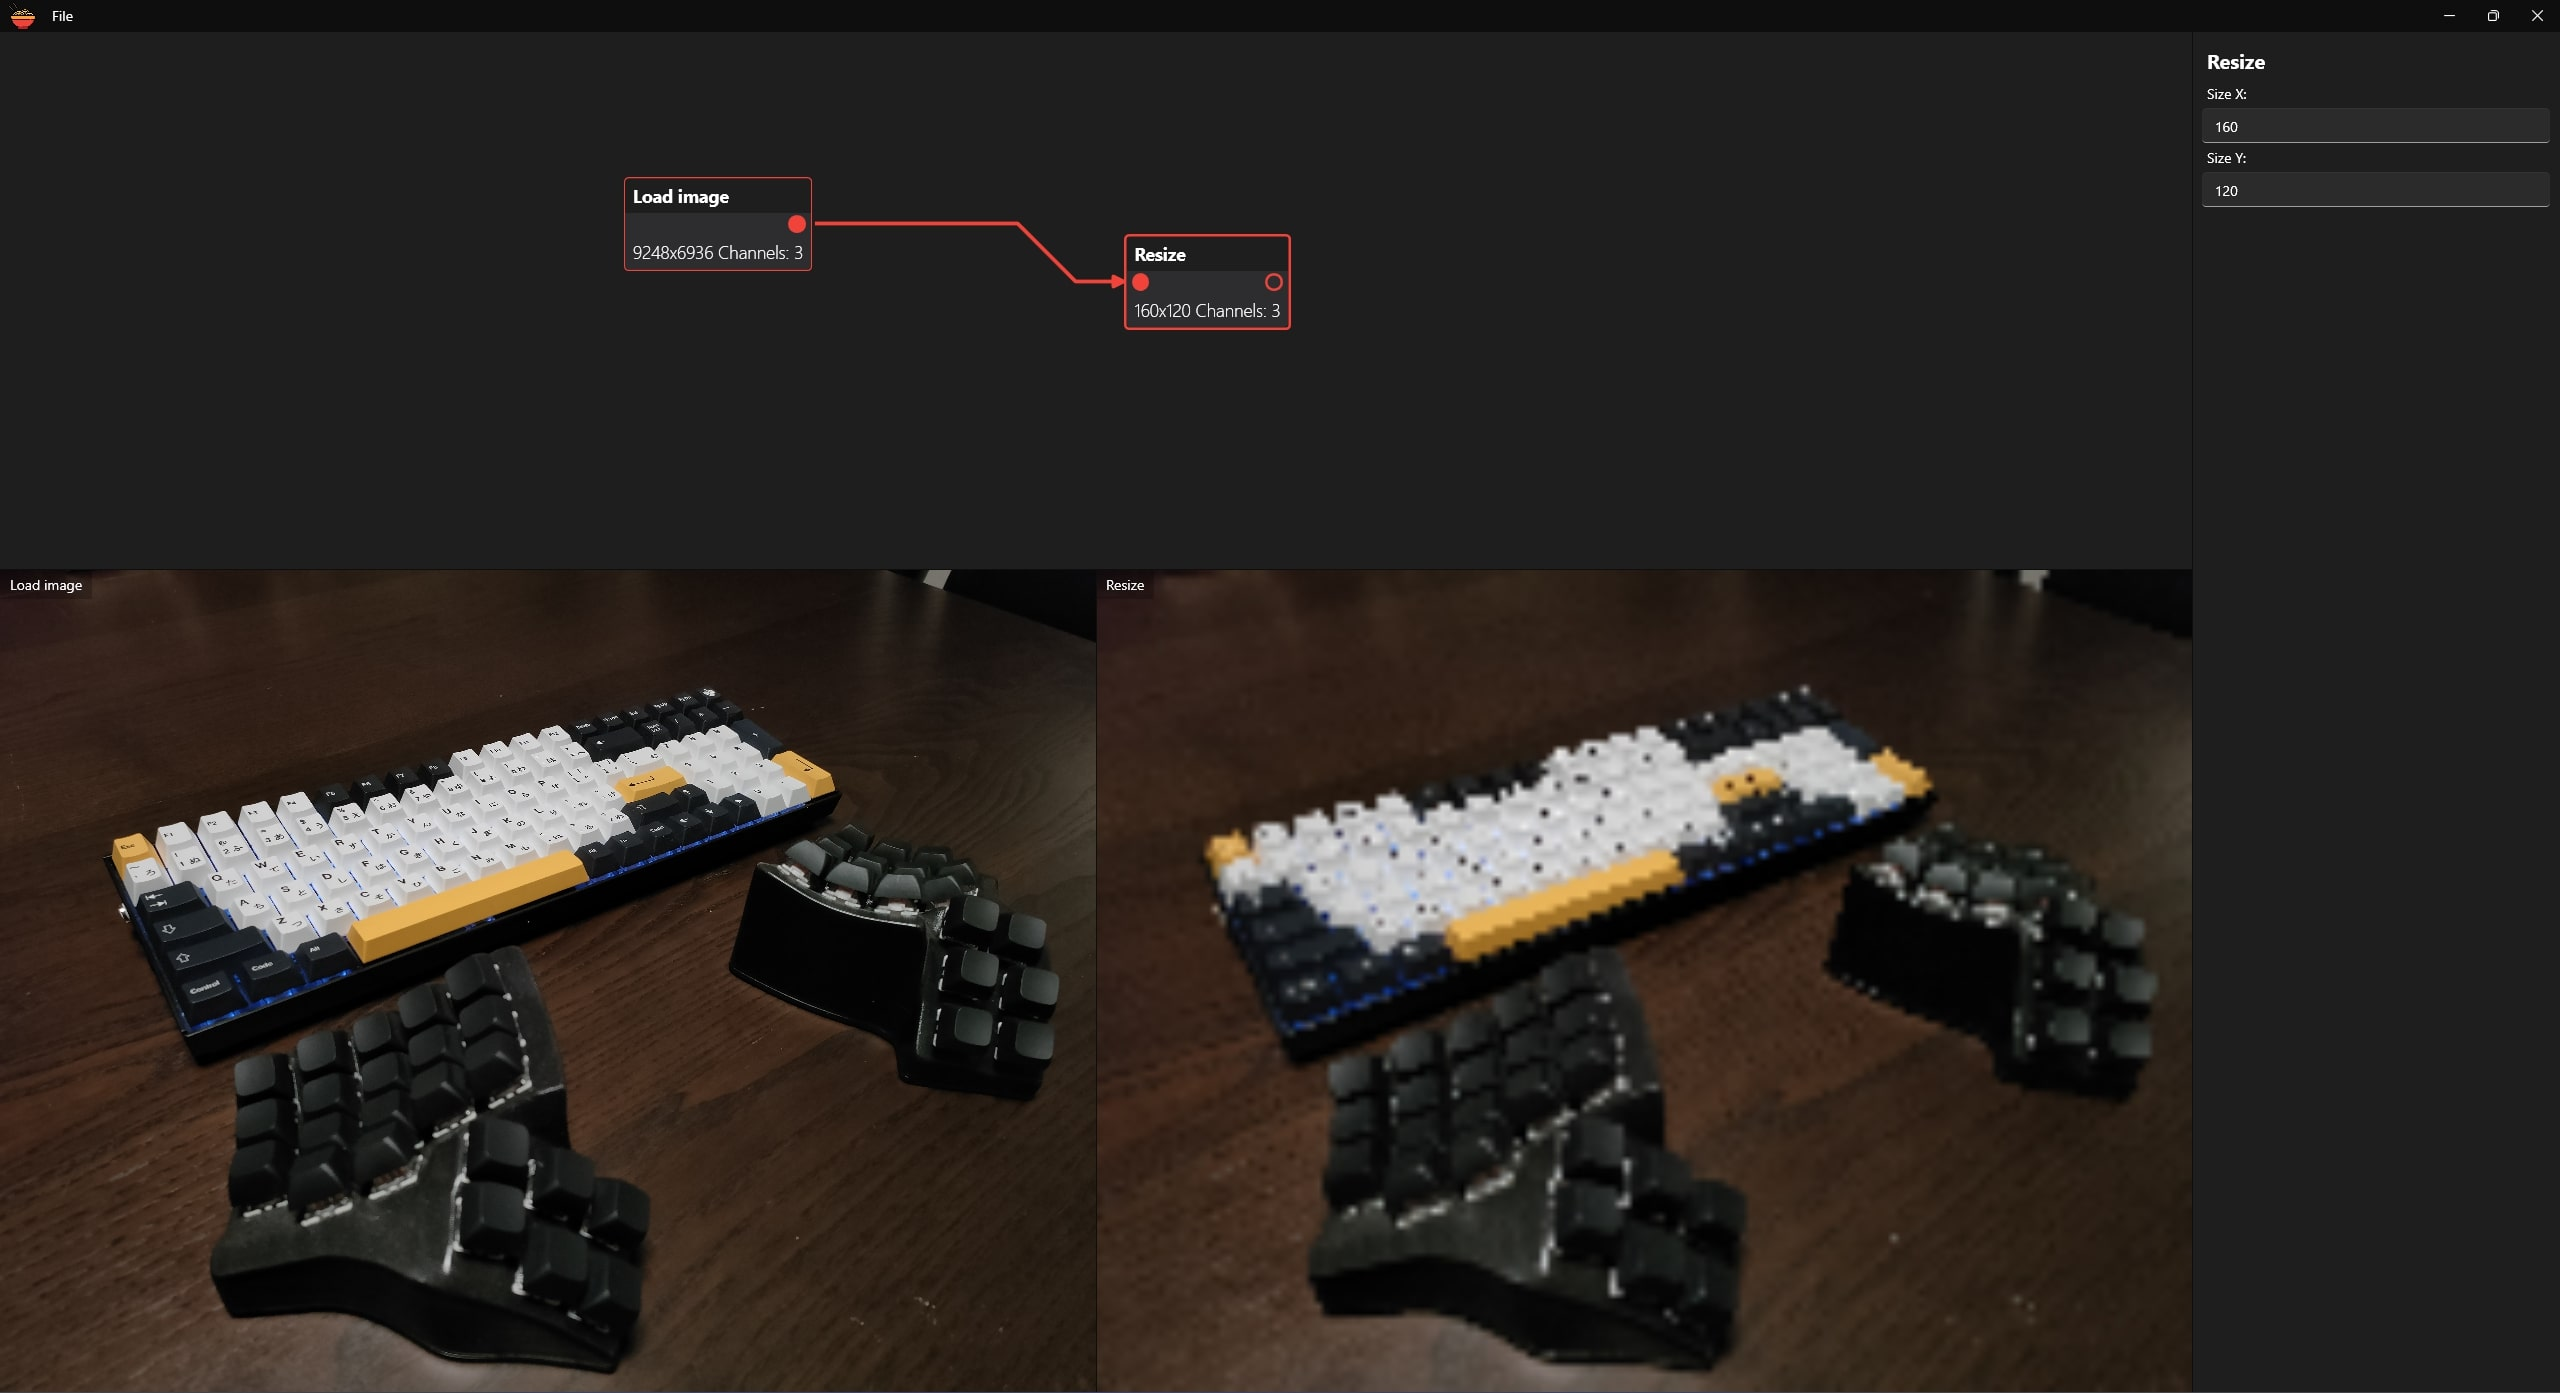
\includegraphics[width=1\linewidth]{images/Picture26.jpg}
    \caption{Operacja \textit{Resize}. Opracowanie własne.}
    \label{fig:resize}
\end{figure} 

\textit{Resize} jest wykonywane przez metodę o tej samej nazwie z biblioteki OpenCV \cite{resize}. Po podaniu nowych wymiarów otrzymujemy obraz stworzony na podstawie oryginalnego ze zmienioną rozdzielczością.